\section{Numerical Implementation in C++}

We have provided a numerical implementation of Gaussian Mixture Models in the C++ language
as part of recent releases of the open source Armadillo C++ linear algebra library~\cite{Armadillo_JOSS_2016,Armadillo_PASC_2017}.
The library can be obtained from \href{http://arma.sourceforge.net}{http://arma.sourceforge.net}.
The implementation contains multi-threaded versions of the Expectation Maximisation (EM) and {\it k}-means training algorithms
(as overviewed in Sections~\ref{sec:param_em} and~\ref{sec:param_km}),
which can considerably speed up training.
% Parallelisation is achieved through refactoring the original EM and {\it k}-means algorithms
% into a MapReduce-like framework~\cite{MapReduce_2004} and employing OpenMP compiler directives~\cite{OpenMP_2007}.

\subsection{Achievable Speedup}

To demonstrate the achievable speedup with the multi-threaded versions of the training algorithms,
we trained a GMM with 100 Gaussians on a recent 16 core machine using synthetic data comprising 1,000,000 samples with 100 dimensions.
10 iterations of the {\it k}-means algorithm and 10 iterations of the EM algorithm were used.
The samples were stored in double precision floating point format, resulting in a total data size of approximately 762~Mb.

Figure~\ref{fig:speedup} shows that a speedup of an order of magnitude is achieved when all 16 cores are used.
We note that the actual speedup is below the idealised linear speedup,
due to memory access contention (stemming from concurrent access to memory by mulitple cores)
as well as overheads related to OpenMP and reduction operations (Section~\ref{sec:param_em_parallel}).


\begin{figure}[!b]
\centering
\begin{minipage}{1\columnwidth}
  \centering
  \begin{minipage}{0.5\textwidth}
    \centering
    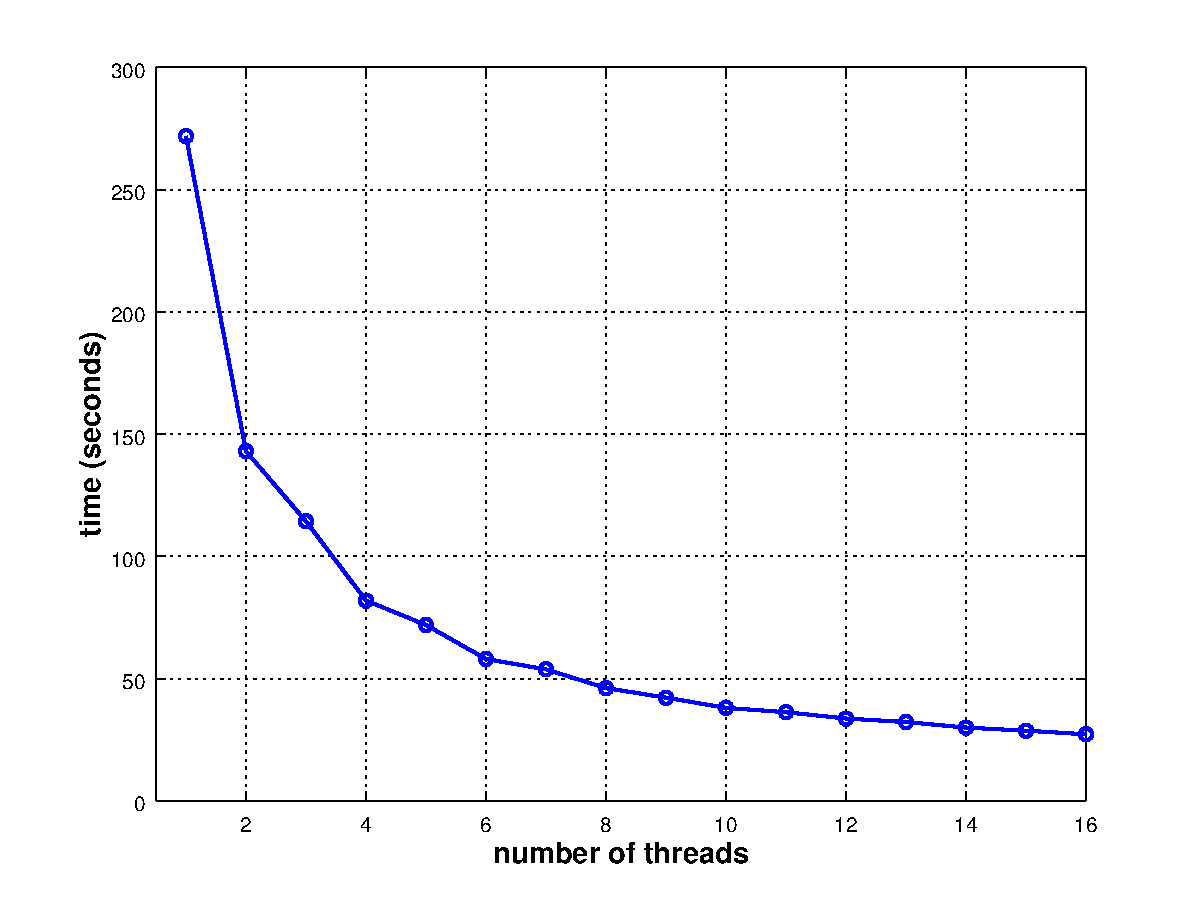
\includegraphics[width=1.1\textwidth]{plot1.pdf}\\
    {(a)}
  \end{minipage}%
  \begin{minipage}{0.5\textwidth}
    \centering
    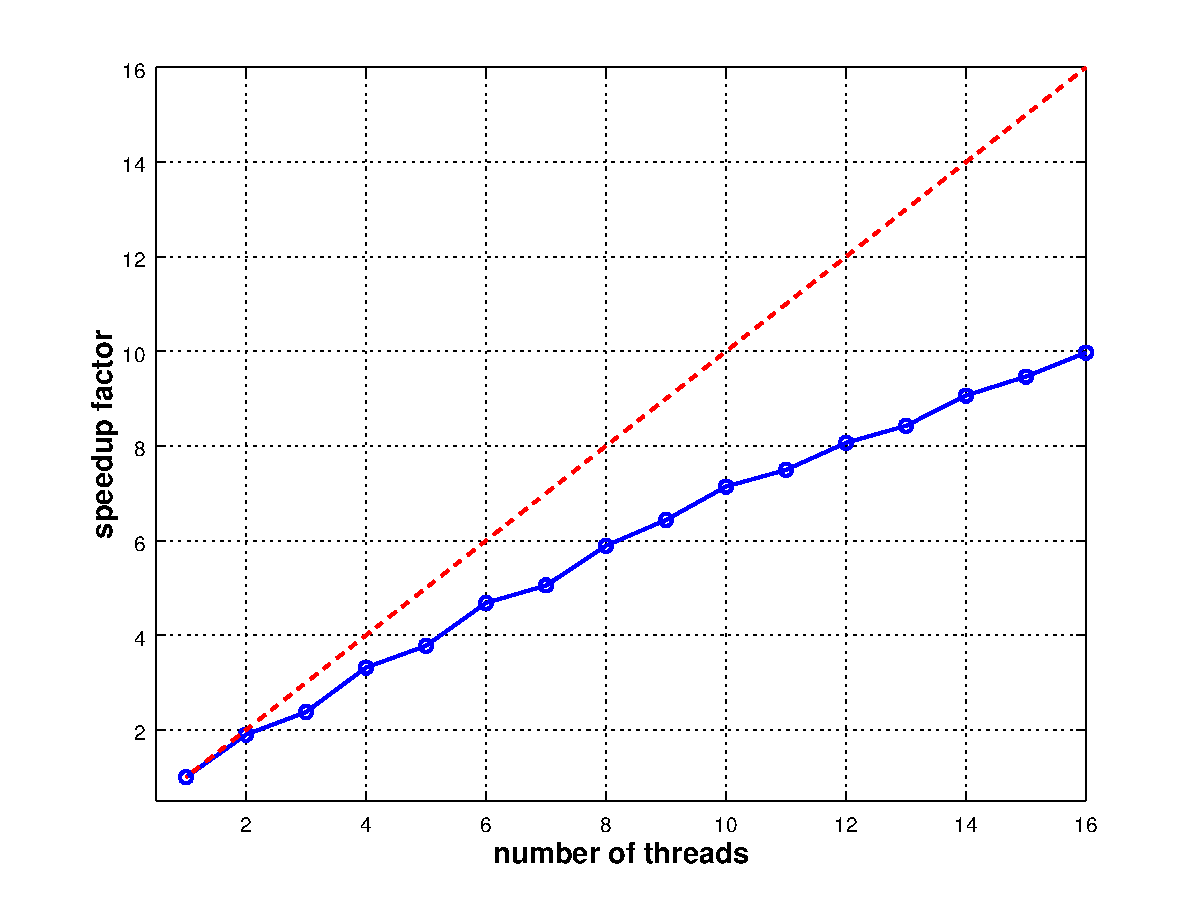
\includegraphics[width=1.1\textwidth]{plot2.pdf}\\
    {(b)}
  \end{minipage}
\end{minipage}
\caption
  {
  Execution characteristics for training a 100 component GMM
  to model synthetic data comprising 1,000,000 samples with 100 dimensions
  using 10 iterations of the {\it k}-means algorithm and 10 iterations of the EM algorithm:
  {\bf (a)}~total time taken depending on the number of threads;
  {\bf (b)}~corresponding speedup factor compared to using one thread (blue line), and idealised linear speedup under the assumption of no overheads and no memory access contention (red dotted line).
  The modelling was done on a machine with dual Intel Xeon E5-2620~v4 CPUs, providing 16 independent processing cores.
  Compilation was done with GCC 5.4 using the following switches: \texttt{-O3 -march=native -fopenmp}.
  }
\label{fig:speedup}
\end{figure}

\subsection{User Accessible Classes and Functions}

The implementation is provided as two user accessible classes within the {\it arma} namespace:
{\it gmm\_diag} and {\it fgmm\_diag}.
The former uses double precision floating point values, while the latter uses single precision floating point values.

For an instance of the double precision {\it gmm\_diag} class named as {\bf M},
its member functions and variables are listed below.
All vectors and matrices refer to corresponding objects from the Armadillo library;
scalars have the type {\it double},
matrices have the type {\it mat},
column vectors have the type {\it vec},
row vectors have the type {\it rowvec},
row vectors of unsigned integers have the type {\it urowvec},
and indices have the type {\it uword} (representing an unsigned integer).
When using the single precision {\it fgmm\_diag} class,
all vector and matrix types have the {\it f} prefix (for example, {\it fmat}),
while scalars have the type {\it float}.
The word ``heft'' is explicitly used in the classes a shorter version of ``weight'', while keeping the same meaning with the context of GMMs.
Figure~\ref{fig:example_usage} contain a complete C++ program which demonstrates usage of the {\it gmm\_diag} class.

\begin{small}
\begin{itemize}

\item
{\bf M.log\_p(V)}\\
return a scalar (double precision floating point value) representing the log-likelihood of column vector {\bf V}

\item
{\bf M.log\_p(V, g)}\\
return a scalar (double precision floating point value) representing the log-likelihood of column vector {\bf V},
according to Gaussian with index {\bf g} (specified as an unsigned integer of type {\it uword})

\item
{\bf M.log\_p(X)}\\
return a row vector (of type {\it rowvec}) containing log-likelihoods of each column vector in matrix {\bf X}


\item
{\bf M.log\_p(X, g)}\\
return a row vector containing log-likelihoods of each column vector in matrix {\bf X},
according to Gaussian with index {\bf g}  (specified as an unsigned integer of type {\it uword})

\item
{\bf M.avg\_log\_p(X)}\\
return a scalar (double precision floating point value) representing the average log-likelihood of all column vectors in matrix {\bf X}

\item
{\bf M.avg\_log\_p(X, g)}\\
return a scalar (double precision floating point value) representing the average log-likelihood of all column vectors in matrix {\bf X},
according to Gaussian with index {\bf g}  (specified as an unsigned integer of type {\it uword})

\item
{\bf M.assign(V, dist\_mode)}\\
return an unsigned integer (of type {\it uword}) representing the index of the closest mean (or Gaussian) to vector {\bf V};\\
parameter {\bf dist\_mode} is one of:

\begin{tabular}{ll}
{\bf eucl\_dist} & Euclidean distance (takes only means into account) \\
{\bf prob\_dist} & probabilistic ``distance'', defined as the inverse likelihood\\
                 & (takes into account means, covariances and hefts)
\end{tabular}

\item
{\bf M.assign(X, dist\_mode)}\\
return a row vector of unsigned integers (of type {\it urowvec}) containing the indices of the closest means (or Gaussians) to each column vector in matrix {\bf X};
parameter {\bf dist\_mode} is either {\bf eucl\_dist} or {\bf prob\_dist}, as per the {\bf .assign()} function above

\item
{\bf M.raw\_hist(X, dist\_mode)}\\
return a row vector of unsigned integers (of type {\it urowvec}) representing the raw histogram of counts;
each entry is the number of counts corresponding to a Gaussian;
each count is the number times the corresponding Gaussian was the closest to each column vector in matrix {\bf X};
parameter {\bf dist\_mode} is either {\bf eucl\_dist} or {\bf prob\_dist}, as per the {\bf .assign()} function above

\item
{\bf M.norm\_hist(X, dist\_mode)}\\
similar to the {\bf .raw\_hist()} function above; return a row vector (of type {\it rowvec}) containing normalised counts; the vector sums to one;
parameter {\bf dist\_mode} is either {\bf eucl\_dist} or {\bf prob\_dist}, as per the {\bf .assign()} function above

\item
{\bf M.generate()}\\
return a column vector representing a random sample generated according to the model's parameters

\item
{\bf M.generate(N)}\\
return a matrix containing {\bf N} column vectors, with each vector representing a random sample generated according to the model's parameters

\item
{\bf M.save(filename)}\\
save the model to a file

\item
{\bf M.load(filename)}\\
load the model from a file

\item
{\bf M.n\_gaus()}\\
return an unsigned integer (of type {\it uword}) containing the number of means/Gaussians in the model

\item
{\bf M.n\_dims()}\\
return an unsigned integer (of type {\it uword}) containing the dimensionality of the means/Gaussians in the model

\item
{\bf M.reset(n\_dims, n\_gaus)}\\
set the model to have dimensionality {\bf n\_dims}, with {\bf n\_gaus} number of Gaussians, specified as unsigned integers of type {\it uword};
all the means are set to zero, all diagonal covariances are set to one, and all the hefts (weights) are set to be uniform

\item
{\bf M.means}\\
read-only matrix (of type {\it mat}) containing the means (centroids), stored as column vectors

\item
{\bf M.dcovs}\\
read-only matrix (of type {\it mat}) containing the diagonal covariances, with the set of diagonal covariances for each Gaussian stored as a column vector

\item
{\bf M.hefts}\\
read-only row vector (of type {\it rowvec}) containing the hefts (weights)

\item
{\bf M.set\_means(X)}\\
set the means (centroids) to be as specified in matrix {\bf X}, with each mean (centroid) stored as a column vector;
the number of means and their dimensionality must match the existing model

\item
{\bf M.set\_dcovs(X)}\\
set the diagonal covariances to be as specified in matrix {\bf X}, with the set of diagonal covariances for each Gaussian stored as a column vector;
the number of diagonal covariance vectors and their dimensionality must match the existing model

\item
{\bf M.set\_hefts(V)}\\
set the hefts (weights) of the model to be as specified in row vector {\bf V};
the number of hefts must match the existing model

\item
{\bf M.set\_params(means, dcovs, hefts)}\\
set all the parameters at the same time, using matrices denoted as {\bf means} and {\bf dcovs} as well as the the row vector denoted as {\bf hefts};
the layout of the matrices is as per the {\bf .set\_means()} and {\bf .set\_dcovs()} functions above;
the number of Gaussians and dimensionality can be different from the existing model

\item
{\bf M.learn(data, n\_gaus, dist\_mode, seed\_mode, km\_iter, em\_iter, var\_floor, print\_mode)}\\
learn the model parameters via the {\it k}-means and/or EM algorithms,
and return a boolean value, with {\it true} indicating success, and {\it false} indicating failure;
the parameters have the following meanings:

\begin{enumerate}[{$\cdot$}]
\item
{\bf data}\\
matrix (of type {\it mat}) containing training samples; each sample is stored as a column vector

\item
{\bf n\_gaus}\\
set the number of Gaussians to {\bf n\_gaus};
to help convergence, it is recommended that the given {\bf data} matrix (above)
contains at least 10 samples for each Gaussian

\item
{\bf dist\_mode}\\
specifies the distance used during the seeding of initial means and {\it k}-means clustering:

\begin{tabular}{ll}
{\bf eucl\_dist} & Euclidean distance\\
{\bf maha\_dist} & Mahalanobis distance, which uses a global diagonal covariance matrix\\
                 & estimated from the given training samples
\end{tabular}

\item
{\bf seed\_mode}\\
specifies how the initial means are seeded prior to running {\it k}-means and/or EM algorithms:

\begin{tabular}{ll}
{\bf keep\_existing} & keep the existing model (do not modify the means, covariances and hefts) \\
{\bf static\_subset} & a subset of the training samples (repeatable) \\
{\bf random\_subset} & a subset of the training samples (random) \\
{\bf static\_spread} & a maximally spread subset of training samples (repeatable) \\
{\bf random\_spread} & a maximally spread subset of training samples (random start)
\end{tabular}

Note that seeding the initial means with {\bf static\_spread} and {\bf random\_spread}
can be more time consuming than with {\bf static\_subset} and {\bf random\_subset}.
These seed modes are inspired by the so-called {\it k-means++} approach~\cite{Arthur_2007}, with the aim to improve clustering quality.

\item
{\bf km\_iter}\\
the maximum number of iterations of the {\it k}-means algorithm; this is data dependent, but typically 10 iterations are sufficient

\item
{\bf em\_iter}\\
the maximum number of iterations of the EM algorithm; this is data dependent, but typically 5 to 10 iterations are sufficient

\item
{\bf var\_floor}\\
the variance floor (smallest allowed value) for the diagonal covariances; setting this to a small non-zero value can help with convergence and/or better quality parameter estimates

\item
{\bf print\_mode}\\
boolean value (either {\it true} or {\it false}) which enables/disables the printing of progress during the {\it k}-means and EM algorithms 

\end{enumerate}


\end{itemize}
\end{small}



\begin{figure}
\hrule
\vspace{1ex}
\centering
% BeraMono
% DejaVu Sans Mono
% KP Monospaced
% LuxiMono
% Inconsolata
%\begin{Verbatim}
%\begin{Verbatim}[fontsize=\footnotesize,fontseries=b]
\begin{Verbatim}[fontfamily=fvm,fontsize=\footnotesize]
#include <armadillo>

using namespace arma;

int main()
  {
  // create synthetic data with 2 Gaussians
  
  uword d = 5;       // dimensionality
  uword N = 10000;   // number of samples (vectors)
  
  mat data(d, N, fill::zeros);
  
  vec mean0 = linspace<vec>(1,d,d);
  vec mean1 = mean0 + 2;
  
  uword i = 0;
  
  while(i < N)
    {
    if(i < N)  { data.col(i) = mean0 + randn<vec>(d); ++i; }
    if(i < N)  { data.col(i) = mean0 + randn<vec>(d); ++i; }
    if(i < N)  { data.col(i) = mean1 + randn<vec>(d); ++i; }
    }
  
  
  // model the data as a GMM with 2 Gaussians
  
  gmm_diag model;
  
  bool status = model.learn(data, 2, maha_dist, random_subset, 10, 5, 1e-10, true);
  
  if(status == false)  { cout << "learning failed" << endl; }
  
  model.means.print("means:");
  
  double overall_likelihood = model.avg_log_p(data);
  
  rowvec     set_likelihood = model.log_p( data.cols(0,9) );
  double  scalar_likelihood = model.log_p( data.col(0)    );
  
  uword   gaus_id  = model.assign( data.col(0),    eucl_dist );
  urowvec gaus_ids = model.assign( data.cols(0,9), prob_dist );
  
  urowvec hist1 = model.raw_hist (data, prob_dist);
   rowvec hist2 = model.norm_hist(data, eucl_dist);
  
  model.save("my_model.gmm");
  
  mat dcovs2 = model.dcovs + 0.1;
  
  model.set_dcovs(dcovs2);
  
  return 0;
  }
\end{Verbatim}
\vspace{-1ex}
\hrule
\vspace{0.5ex}
\caption
  {
  An example C++ program which demonstrates usage of the {\it gmm\_diag} class.
  }
\label{fig:example_usage}
\end{figure}
